\section[]{\textgreek{Γενικά για τη σύζευξη πινάκων}}


\begin{frame}[t, fragile, shrink]
\frametitle{Σκοπός του μαθήματος}
\begin{minipage}{\wE}
\begin{enumerate} \itemsep 9pt % [<+->] \pause \large
  \item Εκτελείτε ερωτήματα ανάσυρσης δεδομένων από πολλούς πίνακες.
  \item Εκτελείτε ερωτήματα που αντιστοιχούν στις σχεσιακές πράξεις καρτεσιανού γινομένου
        και σύζευξης.
  \item Εφαρμόζετε κατάλληλες συνδέσεις ({\sq JOIN}) πινάκων.        
  \item Αντιληφθείτε τις διαφορές και ομοιότητες ανάμεσα στους διαφορετικούς τύπους
        συζεύξεων.
\end{enumerate}
\end{minipage}
\end{frame}


\begin{frame}[t, fragile, shrink]
\frametitle{Το σχήμα της βάσης {\en company}}
\begin{align*}
  departments & (\underline{depid}, depname, manager) \\
  employees   & (\underline{empid}, firstname, lastname, depid, salary, hiredate) \\
  projects    & (\underline{proid}, title, budget, startdate, enddate, progress) \\
  workson     & (\underline{empid}, \underline{proid})
\end{align*}
\begin{itemize}
  \item {\ra departments}, τα τμήματα της εταιρείας
  \item {\ra employees}, οι υπάλληλοι της εταιρείας
  \item {\ra projects}, τα έργα που εκτελεί η εταιρεία
  \item {\ra workson}, η απασχόληση των υπαλλήλων στα έργα
\end{itemize}
\end{frame}



\begin{frame}[t, fragile, shrink]
\frametitle{Το σχήμα της βάσης {\en company}}
\begin{minipage}{\wE}
\begin{columns}[t]
\begin{column}{0.55\linewidth}
\begin{center}
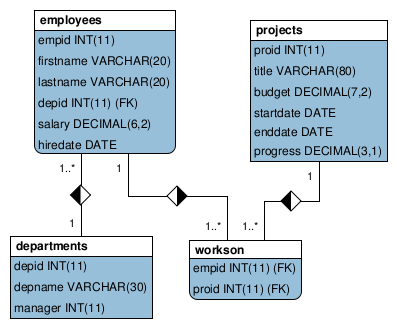
\includegraphics[scale=0.5]{../common/companyER.png}
\end{center}
\end{column}
\begin{column}{0.4\linewidth}
\begin{center}
\begin{itemize}
  \item {\ra departments}, τα τμήματα της εταιρείας
  \item {\ra employees}, οι υπάλληλοι της εταιρείας
  \item {\ra projects}, τα έργα που εκτελεί η εταιρεία
  \item {\ra workson}, η απασχόληση των υπαλλήλων στα έργα
\end{itemize}
\end{center}
\end{column}
\end{columns}
\end{minipage}
\end{frame}


\begin{frame}[t, fragile, shrink]
\frametitle{Πρωτεύοντα και ξένα κλειδιά}
\begin{minipage}{\wE}
\begin{enumerate} \itemsep 6pt % [<+->] \pause
  \item Κάθε πίνακας έχει ένα {\crr πρωτεύον κλειδί}.
  \item Το {\crr πρωτεύον κλειδί} μπορεί να είναι απλό (ένα πεδίο), ή σύνθετο
        (συνδυασμός πεδίων).
  \item Κάθε εγγραφή ενός πίνακα μπορεί να προσδιοριστεί με τη χρήση του
        πρωτεύοντος κλειδιού.
  \item Η σύνδεση δεδομένων από διαφορετικούς πίνακες {\bbl σύζευξη}
        γίνεται (συνήθως) με τη χρήση του {\crr ξένου κλειδιού},
  \item Ένας πίνακας μπορεί να έχει πολλά ξένα κλειδιά ή  να μην έχει κανένα.
\end{enumerate}
\end{minipage}
\end{frame}


\begin{frame}[t, fragile, shrink]
\frametitle{Συσχέτιση {\en departments} και {\en employees} Ν:1}
\begin{itemize} \itemsep 6pt
  \item Ο πίνακας {\ra departments} έχει {\crr πρωτεύον κλειδί} το πεδίο {\ra depid}.
  \item Ο πίνακας {\ra employees} έχει {\crr πρωτεύον κλειδί} το πεδίο {\ra empid}.
  \item Ο πίνακας {\ra employees} έχει {\crr ξένο κλειδί} το πεδίο {\ra depid},
        το οποίο παίρνει τιμές που {\bbl αναφέρονται} στις τιμές του πεδίου
        {\ra depid} του πίνακα {\ra departments}:
        \[ departments.depid = employees.depid \]
\end{itemize}
\pause
\begin{minipage}{\wE}
\begin{itemize} 
  \item Το πεδίο {\ra employees.depid}  {\crr δεν είναι πρωτεύον κλειδί}
        και δεν παίρνει μοναδικές τιμές: πολλοί υπάλληλοι εργάζονται
        στο ίδιο τμήμα.
  \item Οι πίνακες {\ra departments} και {\ra employees}  συσχετίζονται μεταξύ τους
        με συσχέτιση {\cee Πολλά προς Ένα}.
\end{itemize}
\end{minipage}
\end{frame}


\begin{frame}[t, fragile, shrink]
\frametitle{Συσχέτιση {\en departments - employees} }
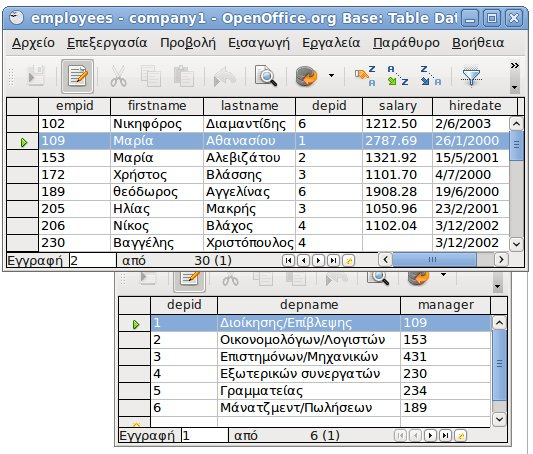
\includegraphics[scale=0.65]{company1-relationship.jpg} \\
\bigskip
\begin{minipage}{\wE}

\end{minipage}
\end{frame}

\begin{frame}[t, fragile, shrink]
\frametitle{Συσχέτιση {\en departments} και {\en employees} 1:1}
\begin{itemize}
  \item Ο πίνακας {\ra departments} έχει {\cee πρωτεύον κλειδί} το πεδίο {\ra depid}.
  \item Ο πίνακας {\ra employees} έχει {\cee πρωτεύον κλειδί} το πεδίο {\ra empid}.
  \item Ο πίνακας {\ra departments} έχει {\cee ξένο κλειδί} το πεδίο {\ra manager},
        το οποίο παίρνει τιμές που {\bbl αναφέρονται} στις τιμές του πεδίου
        {\ra empid} του πίνακα {\ra employees}:
        \[ departments.manager = employees.empid \]
\end{itemize}
\pause
\begin{minipage}{\wE}
\begin{itemize} 
  \item Το πεδίο {\ra departments.manager}  {\cee δεν είναι πρωτεύον κλειδί}
        αλλά παίρνει μοναδικές τιμές ({\sq UNIQUE}).
  \item Οι πίνακες {\ra departments} και {\ra employees}  συσχετίζονται μεταξύ τους
        με συσχέτιση {\cee  Ένα προς Ένα}.
\end{itemize}
\end{minipage}
\end{frame}




\begin{frame}[t, fragile, shrink]
\frametitle{Συσχέτιση {\en employees} και {\en projects} Ν:Ν}
\begin{minipage}{\wE}
\begin{enumerate} \itemsep 6pt % [<+->] \pause 
  \item Ο πίνακας {\ra projects} έχει {\crr πρωτεύον κλειδί} το πεδίο {\ra proid}.
  \item Ο πίνακας {\ra workson} έχει {\crr πρωτεύον κλειδί} το συνδυασμό των πεδίων
        {\ra empid} και  {\ra proid} ({\crr σύνθετο κλειδί}).
  \item Το πεδίο {\ra empid} είναι {\cee ξένο κλειδί} στον πίνακα {\ra workson}
        και αναφέρεται στο πεδίο {\ra employees.empid}.
  \item Το πεδίο {\ra proid} είναι {\crr ξένο κλειδί} στον πίνακα {\ra workson}
        και αναφέρεται στο πεδίο {\ra projects.proid}.  
  \item Ένας υπάλληλος απασχολείται σε πολλά έργα, ένα έργο απασχολεί
        πολλούς υπαλλήλους,  επομένως η συσχέτιση είναι {\cee Πολλά προς Πολλά}.
  \item Η σύζευξη των πινάκων {\ra employees} και {\ra projects} \\ γίνεται
        μέσω του πίνακα {\ra workson}.
\end{enumerate}
\end{minipage}
\end{frame}



\begin{frame}[t, fragile, shrink]
\frametitle{Το σχήμα της βάσης {\en company (MySQL)}}
\begin{minipage}{\wE}
\begin{columns}
\begin{column}{0.55\linewidth}
\begin{center}
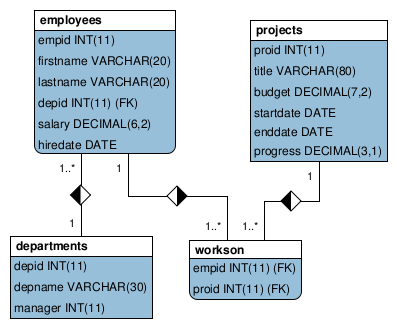
\includegraphics[scale=0.5]{../common/companyER.png}
\end{center}
\end{column}
\begin{column}{0.4\linewidth}
\begin{center}
\begin{itemize}
  \item {\ra departments}, τα τμήματα της εταιρείας
  \item {\ra employees}, οι υπάλληλοι της εταιρείας
  \item {\ra projects}, τα έργα που εκτελεί η εταιρεία
  \item {\ra workson}, η απασχόληση των υπαλλήλων στα έργα
\end{itemize}
\end{center}
\end{column}
\end{columns}
\end{minipage}
\end{frame}


\begin{frame}[t, fragile, shrink]
\frametitle{Το σχήμα της βάσης {\en company (.odp)} }
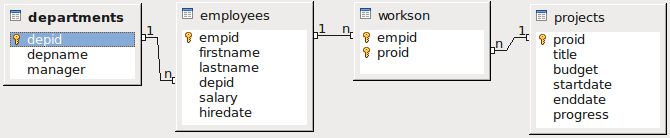
\includegraphics[scale=0.65]{../common/company1-REL-odp.png} \\
\bigskip
\begin{minipage}{0.92\textwidth}
\begin{itemize} \itemsep 9pt
  \item {\ra departments}, τα τμήματα της εταιρείας
  \item {\ra employees}, οι υπάλληλοι της εταιρείας
  \item {\ra projects}, τα έργα που εκτελεί η εταιρεία
  \item {\ra workson}, η απασχόληση των υπαλλήλων στα έργα
\end{itemize}
\end{minipage}
\end{frame}
